% Made up for the tikra benchmark.
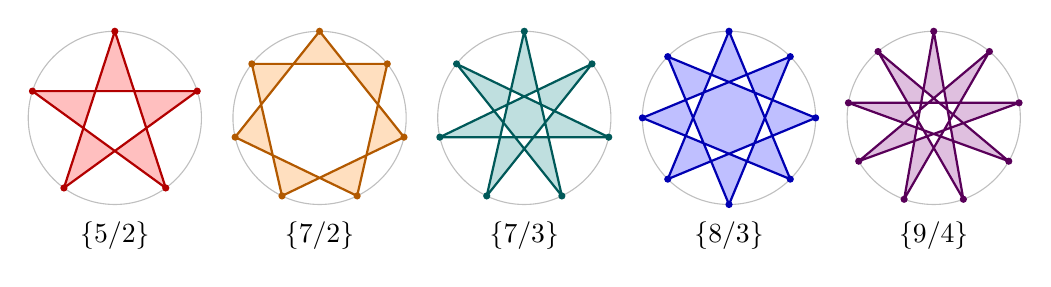
\begin{tikzpicture}[line join=round]
  \foreach \n/\m/\c [count=\i from 0] in {5/2/red, 7/2/orange, 7/3/teal, 8/3/blue, 9/4/violet} {
    \begin{scope}[xshift=\i*2.6cm]
      \draw[gray!50] (0,0) circle (1.1);
      \filldraw[\c!70!black, thick, fill=\c!25, even odd rule]
        (90:1.1) \foreach \k in {1,...,\n} { -- ({90+360*\m*\k/\n}:1.1) } -- cycle;
      \foreach \k in {1,...,\n} { \fill[\c!70!black] ({90+360*\k/\n}:1.1) circle (1.3pt); }
      \node[below] at (0,-1.2) {$\{\n/\m\}$};
    \end{scope}
  }
\end{tikzpicture}
